


\begin{document}

This section details the experimental implementation of the two differential amplifiers, the resistively loaded and active loaded. The power supplies and analysis were implemented using the Digilent Analog Discovery kit.

The experimental circuit can be seen Figure \ref{fig:expercircuit}.

\begin{figure}[H]
	\begin{center}
		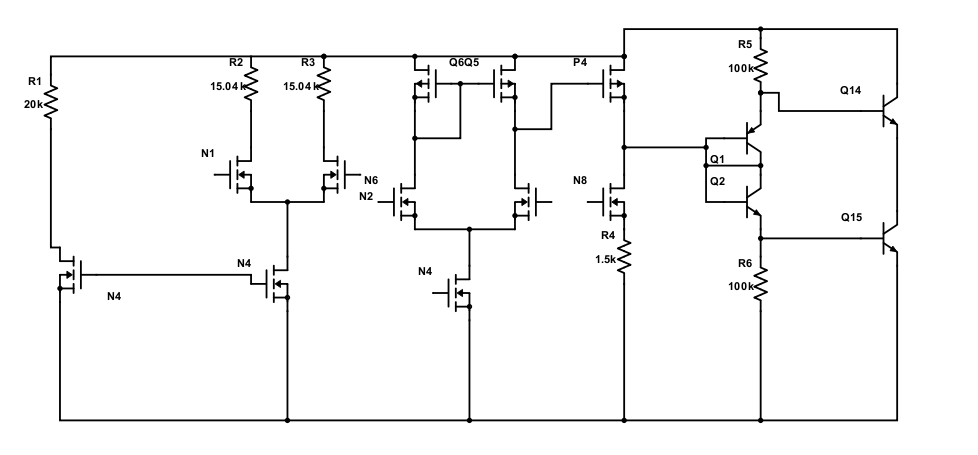
\includegraphics[scale=.40]{ExperimentalImplementation/task4.png}
		\caption{Experimental operational amplifier}
		\label{fig:expercircuit}
	\end{center}
\end{figure}
The simulated circuit, when constructed, failed to meet both the final differential gain output of 46 dB as well as the CMRR of 60 dB. As a result the final circuit design was changed to the op amp design \#1, which can be seen in Figure \ref{fig:expercircuit}. Further details on why design was changed can be found in the Discussion section.

The DC bias conditions were measured using a DT830B DVM. Nodal voltages were measured in reference to ground and current was measured by wiring the DVM in series while in ammeter mode. The bias conditions were measured while both input nodes to the circuit were grounded. The final measured values can be seen in Table \ref{tab:expdc}.


\begin{table}[H]
	\centering
	\caption{Experimental DC values}
	\label{tab:expdc}
	\begin{tabular}{|l|l|}
		\hline
		\textbf{DC Bias Conditions} &           \\ \hline
		Vref                        & -3.03V    \\ \hline
		Iref                        & 396$\mu$A \\ \hline
		D1                          & 2.01V     \\ \hline
		D2                          & 1.99V     \\ \hline
		S                           & -2.04V    \\ \hline
		OutCS                       & 100mV      \\ \hline
	\end{tabular}
\end{table}

Notably, the voltage at the "OutCS" node should be zero. In the default state, the offset at that node was measured to be 2.5V. A potentiometer was used as the source degeneration resistance for the common source amplifier. This pot was varied until the offset was nulled out and the final resistance value required was found to be 1.5k$\Omega$. The range of operation for the circuit can be seen in Figure \ref{fig:vtc}.


\begin{figure}[H]
	\begin{center}
		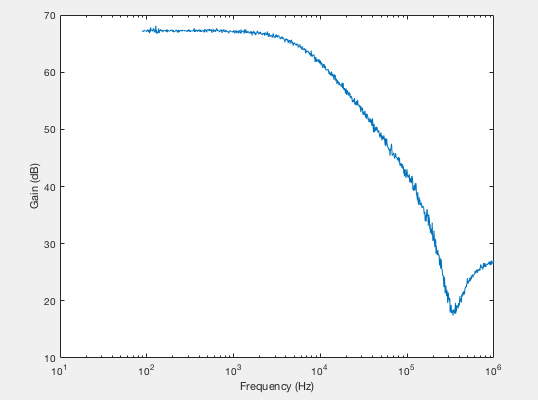
\includegraphics[scale=.40]{ExperimentalImplementation/Ad_final.png}
		\caption{Experimental range of operation}
		\label{fig:vtc}
	\end{center}
\end{figure}

The range of operation is extremely 




 The final differential gain can be seen in Figure \ref{fig:finalAD}.

\begin{figure}[H]
	\begin{center}
		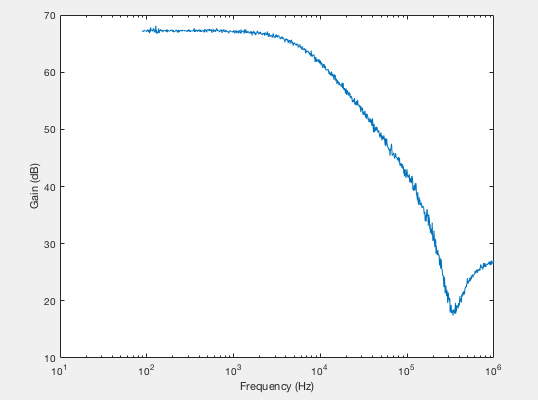
\includegraphics[scale=.40]{ExperimentalImplementation/Ad_final.png}
		\caption{Experimental differential gain}
		\label{fig:finalAD}
	\end{center}
\end{figure}

The max differential gain can be seen to be 67 dB. This is more than 20 dB greater than the minimum specification. Even more noteworthy, however, is the fact that the gain is not unity gain stable. The gain plot, at least within the range of 100 Hz to 1MHz, never crosses the 0 dB point. As a result, the amplifier is said to not be unity gain stable. This can be remedied by including a capacitor at the output stage and will be done during Task 5. The phase of the differential gain phase can be seen in Figure \ref{fig:adphase}. 

\begin{figure}[H]
	\begin{center}
		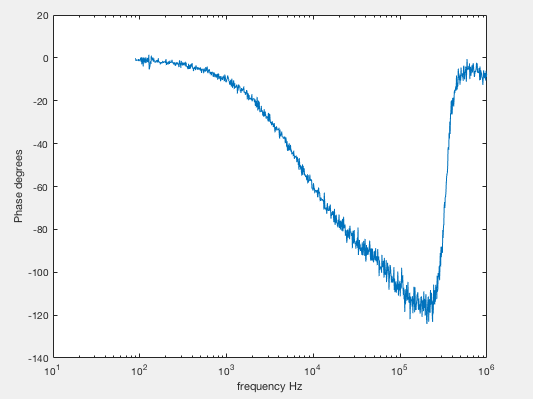
\includegraphics[scale=.40]{ExperimentalImplementation/Ad_phase.png}
		\caption{Experimental differential gain phase}
		\label{fig:adphase}
	\end{center}
\end{figure}

The phase can be seen to return to unity after 100kHz. This is also a result of the lack of frequency compensation. Notably, the phase mirrored that of the simulated design quite well. 
 


 
\end{document}


